
%......................................
\subsubsection{The Stenberg macro-element} 

\begin{center}
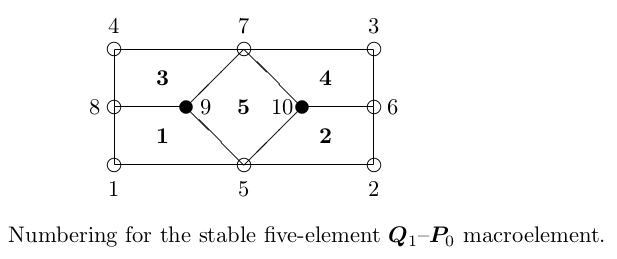
\includegraphics[width=5cm]{images/meshtopos/elsw}
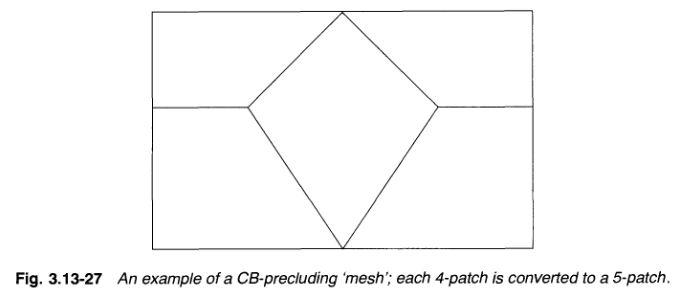
\includegraphics[width=5cm]{images/meshtopos/grsa}\\
{\captionfont Left: Fig 3.12 of Elman et al book \cite{elsw}.
Right: Taken from Gresho \& Sani's book \cite{grsa}: "For fans of $Q_1Q_0$ who want 
guaranteed optimal convergence of both u and p (with however larger error 
constants caused by the distorted shapes?), one way to assure this is
to discretise via the macro elements above, each composed of five $Q_1Q_0$
quadrilaterals. Such checkerboard-killer meshes have been employed in practice
by (at least) Bath\'e \cite{chba93}. Both the macro-element and the proof are
due to Stenberg \cite{sten84}."}
\end{center}

\begin{center}
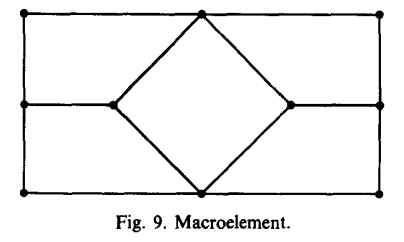
\includegraphics[width=5cm]{images/meshtopos/chba93}\\
{\captionfont Taken from Chapelle \& Bathe \cite{chba93}: "the numerical inf-sup test is passed for this mesh and in fact,
this behavior was proven analytically (see Brezzi \& Fortin \cite{brfo}, see also Le Tallec \& Ruas \cite{leru86}).}
\end{center}

\begin{center}
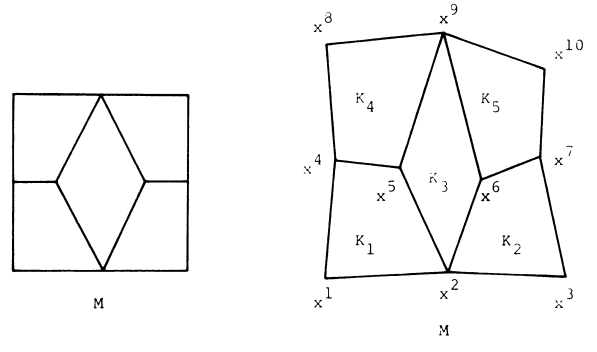
\includegraphics[width=5cm]{images/meshtopos/sten84}
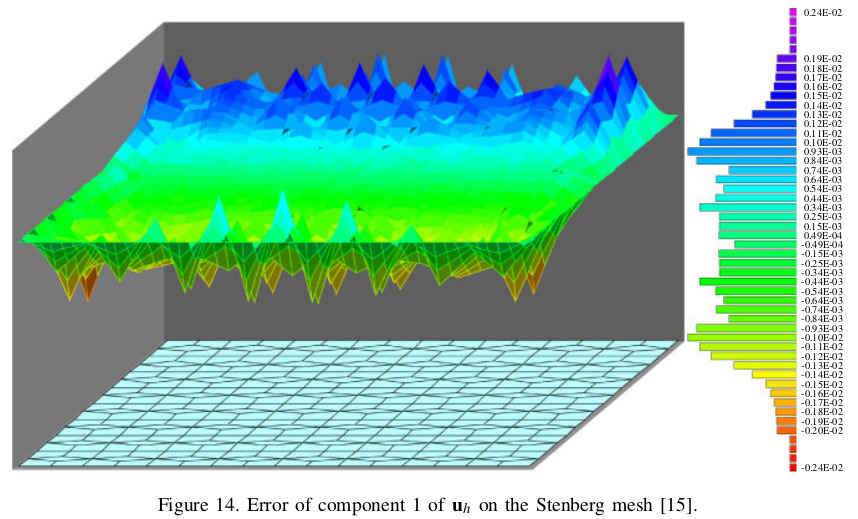
\includegraphics[width=5cm]{images/meshtopos/qizh07}\\
{\captionfont Left: Taken from Stenberg (1984) \cite{sten84}. 
Right: Taken from Qin \& Zhang (2007) \cite{qizh07}.}
\end{center}

%......................................
\subsubsection{The Le Tallec macro-element} 

\begin{center}
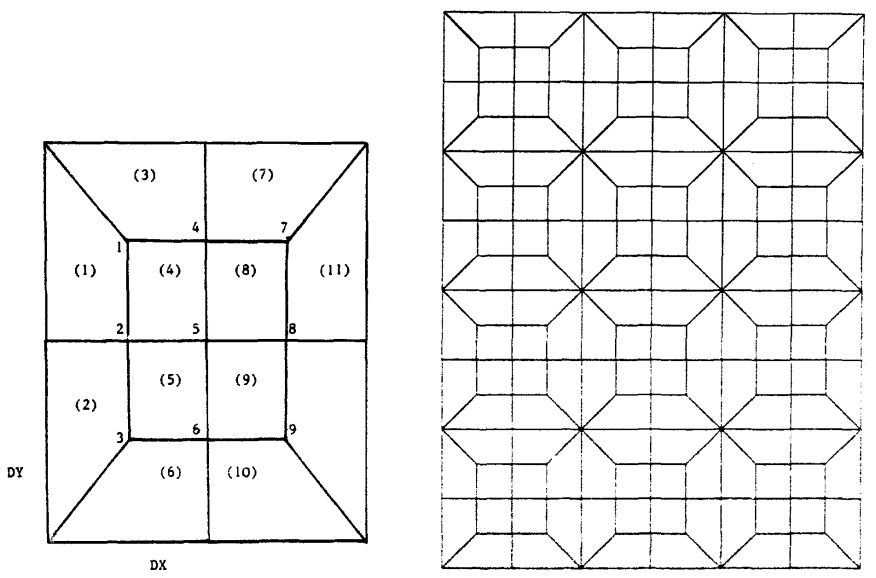
\includegraphics[width=7cm]{images/meshtopos/leta81}\\
{\captionfont Taken from Le Tallec (1981) \cite{leta81}.}
\end{center}
This macro-element has been proven stable in \cite{leta81,leru86}, i.e. it satisfies 
the stability condition (see Section~\ref{ss:pair}).
It is also mentioned in \cite{qizh07}.

%..............................................
\subsubsection{The Qin \& Zhang macro-elements}

In their paper \cite{qizh07} the authors mention the above two macro-elements 
and also introduce three new ones:

\begin{center}
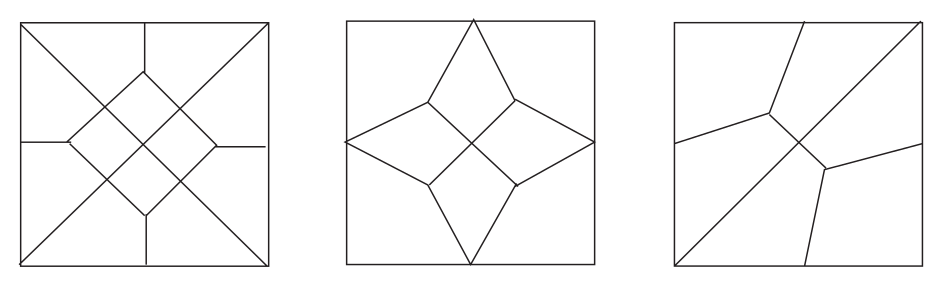
\includegraphics[width=10cm]{images/meshtopos/qizh07b}
\end{center}

They also indicate that although stable, these macro-elements are inferior 
to the above two. 

%..............................................
\subsubsection{New macro-elements ?}

\begin{center}
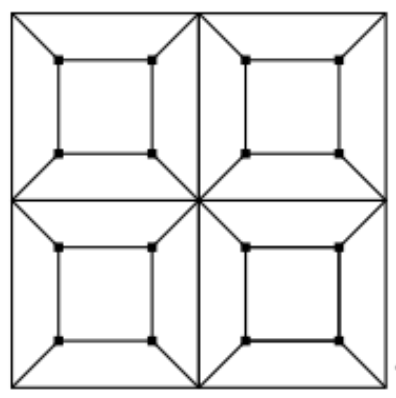
\includegraphics[width=4cm]{images/meshtopos/m21}
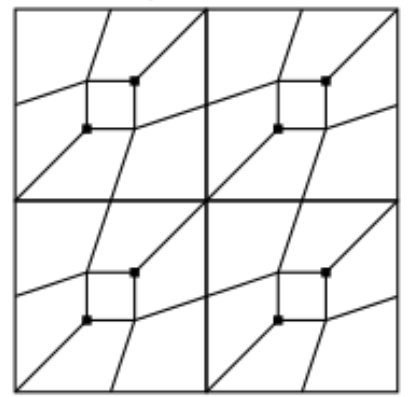
\includegraphics[width=4cm]{images/meshtopos/m22}
\end{center}

I came up with these, no idea whether these are stable/usable or better than the others.






 

